\documentclass[letterpaper,10pt]{article}

\usepackage{titling}
\usepackage{listings}
\usepackage{url}
\usepackage{setspace}
\usepackage{subfig}
\usepackage{sectsty}
\usepackage{pdfpages}
\usepackage{colortbl}
\usepackage{multirow}
\usepackage{multicol}
\usepackage{relsize}
\usepackage{amsmath}
\usepackage{wasysym}
\usepackage{fancyvrb}
\usepackage{amssymb}
\usepackage{ifsym}
\usepackage{amsmath,amssymb,amsthm,graphicx,xspace}
\usepackage[titlenotnumbered,noend,noline]{algorithm2e}
\usepackage[compact]{titlesec}
\usepackage{XCharter}
\usepackage[T1]{fontenc}
\usepackage{tikz}
\usetikzlibrary{arrows,automata,shapes,trees,matrix,chains,scopes,positioning,calc}
\tikzstyle{block} = [rectangle, draw, fill=blue!20, 
    text width=2.5em, text centered, rounded corners, minimum height=2em]
\tikzstyle{bw} = [rectangle, draw, fill=blue!20, 
    text width=4em, text centered, rounded corners, minimum height=2em]

\definecolor{namerow}{cmyk}{.40,.40,.40,.40}
\definecolor{namecol}{cmyk}{.40,.40,.40,.40}

\let\LaTeXtitle\title
\renewcommand{\title}[1]{\LaTeXtitle{\textsf{#1}}}


\newcommand{\handout}[5]{
  \noindent
  \begin{center}
  \framebox{
    \vbox{
      \hbox to 5.78in { {\bf ECE356: Database Systems } \hfill #2 }
      \vspace{4mm}
      \hbox to 5.78in { {\Large \hfill #4  \hfill} }
      \vspace{2mm}
      \hbox to 5.78in { {\em #3 \hfill} }
    }
  }
  \end{center}
  \vspace*{4mm}
}

\newcommand{\lecture}[3]{\handout{#1}{#2}{#3}{Lecture #1}}
\newcommand{\tuple}[1]{\ensuremath{\left\langle #1 \right\rangle}\xspace}

\addtolength{\oddsidemargin}{-1.000in}
\addtolength{\evensidemargin}{-0.500in}
\addtolength{\textwidth}{2.0in}
\addtolength{\topmargin}{-1.000in}
\addtolength{\textheight}{1.75in}
\addtolength{\parskip}{\baselineskip}
\setlength{\parindent}{0in}
\renewcommand{\baselinestretch}{1.5}
\newcommand{\term}{Winter 2018}

\singlespace


\begin{document}

\lecture{ 15 --- Query Processing }{\term}{Jeff Zarnett}

\section*{Query Processing}

Imagine you are given an assignment in a course and you are going to do it now. To get the assignment done, you will probably (1) figure out what exactly the assignment is asking you to do; (2) figure out how you are going to go it (e.g., must do part 1 first because part 2 depends on it...); and finally (3) do it! 

The procedure for the database server to carry out the query are the same~\cite{dsc}:

\begin{enumerate}
	\item Parsing and translation -- interpreting the SQL query in a form the computer can work with.
	\item Optimization -- figuring out how best to carry out the query.
	\item Evaluation -- execution of the query according to the plan just developed.
\end{enumerate}

To break these steps down into more detail, as in~\cite{fds}, the steps are a bit more like this. First, the scanner needs to figure out what are keywords and attribute names and relation names to figure out the text of the query. The parser will then check that it is valid SQL syntax. If so, then it will be validated to make sure that the attribute and relation names are valid inside the schema of the database being queried. Then this query is turned into a query tree or graph, which is used to devise the execution strategy. Then finally we can execute the query.

A quick visual summary of all the steps we are going to go through~\cite{dsc}:
\begin{center}
	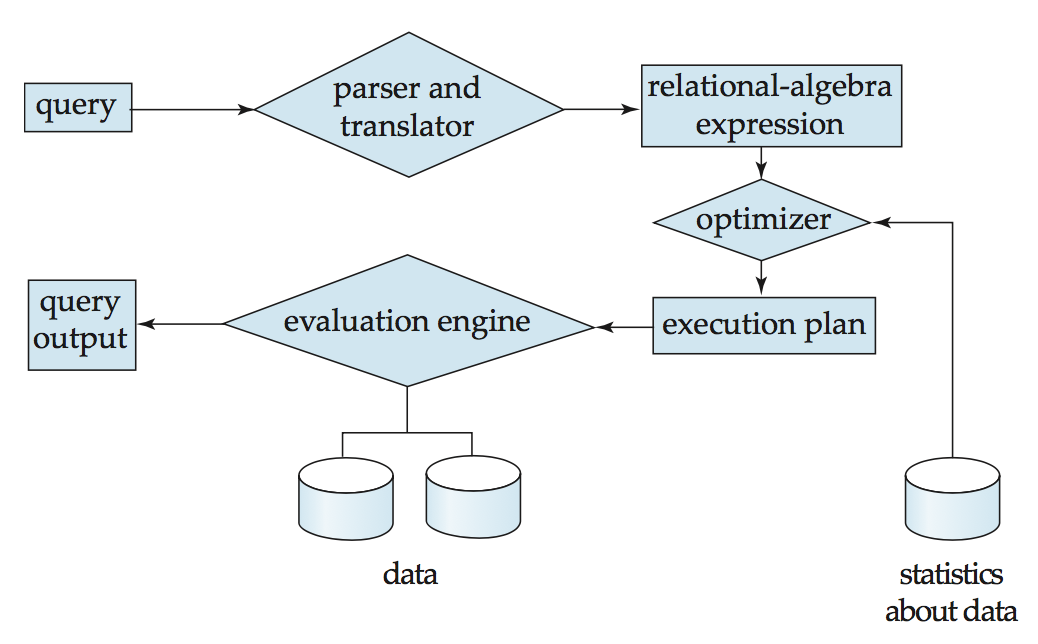
\includegraphics[width=0.5\textwidth]{images/query-processing-overview}
\end{center}

We will not spend time talking about the scanning, parsing, and verification steps of query processing. While they are all very important things and we need them, that is the sort of material that belongs in compiler textbooks and you may have already covered (or at least begun to cover) such material in a compilers course. In the meantime, if a query is syntactically invalid, or contains misspelled attributes, or something to that effect, we can't really do anything with it a query with an error is simply rejected and  goes no further through the process. We therefore will give them no further consideration.

Usually a query is expressed in SQL and that must then be translated into an equivalent relational algebra expression. Complex SQL queries are typically turned into \textit{query blocks}, which are translatable into relation algebra expressions. A query block has a single select-from-where expression, as well as related group-by and having clauses; nested queries are a separate query block~\cite{fds}.

A query like \texttt{SELECT salary FROM employee WHERE salary > 100000;} consists of one query block. The relational algebra for this expression is pretty easy to work out, and it gives us two possibilities. We can select all tuples where salary is more than 100~000 and then perform a projection of the salary field of that result (e.g., throw away the fields we do not need). The alternative is to do the projection of salary first and then perform the selection on the cut-down intermediate relation.

Suppose there is a subquery, like \texttt{SELECT name, street, city, province, postalCode FROM address WHERE id IN (SELECT addressID FROM employee WHERE department = 'Development');}. Then there are two query blocks, one for the subquery and one for the outer query. If there are multiple query blocks, then they do not have to follow the same strategy; they can be optimized separately if desired. 

The relational algebra is not quite enough to actually carry out the operation. What we need instead is a \textit{query execution plan}\footnote{\url{https://www.youtube.com/watch?v=fQk_832EAx4}}. To build that up, each step of the plan needs annotations that specify how to evaluate the operation, including information such as what algorithm or what index to use. An algebraic operation with the associated annotations about how to get it done is called an \textit{evaluation primitive}. The sequence of these primitives forms the plan, that is, how exactly to execute the query~\cite{dsc}. 

If there are multiple possible way to carry out the plan, which there very often are, then the system will need to make some assessment about which plan is the best. It is not expected that users will write optimal queries; instead the database server should choose the best approach via \textit{query optimization}. Optimization is perhaps the wrong name for this because we are not choosing the optimal approach; instead we will make some estimates about the query plans and try to choose the one that is most likely to be best. The subject of query optimization is something we will touch on now, but also come back to when we have more understanding.

\subsection*{Measures of Query Cost}

If you are asked to drive a car from point A to point B and there are multiple routes, you can evaluate your choices. To do so you need to break it down into different sections, such as drive along University Avenue, then get on Highway 85, then merge onto 401... Each segment has a length and a speed, such as knowing that you will drive 4 km along University Avenue and it is signed at 50 km/h (although with red lights and traffic and whatnot the actual average speed may be more like 30 km/h). By combining all of the segments, you get an estimate of how long that particular route will take. If you do this for all routes, you can see which route is the best. 

Of course, it may turn out that real life gets in the way: if there is a crash on the highway, traffic really sucks and your decision that taking this particular route would be fastest turns out to be wrong. Short of being able to see into the future, this is more or less inevitable: estimates are just informed opinions and things may be worse (or better) than expected. 

Where does the time go in executing a query? The biggest component is most likely loading blocks from disk, considering how slow the disk operations are. Although we can improve this via use of SSDs, many large databases still use hard disk drives. CPU speeds are pretty fast, to the point even where memory accesses seem slow from the perspective of the CPU. So, no matter what we do, disk accesses likely account for far more of the time than CPU computation. In reality, CPU time is a nonzero part of query optimization, but we will ignore this (as does~\cite{dsc}) for simplicity's sake and use only the disk accesses to assess cost.

The number of block transfers (data moved in and out of memory) and the number of disk seeks (repositioning where on the disk we are reading from) are the important measures of interest here. SSDs have no seek time and have faster transfer speeds, but the number of block transfers is still relevant. 

\bibliographystyle{alphaurl}
\bibliography{356}


\end{document}
